\begin{frame}[fragile]{What is this course?}

\begin{columns}[T,onlytextwidth]
    \begin{column}{0.35\linewidth}
        \begin{figure}
            \centering
            \resizebox{!}{0.5\textheight}{%
            \begin{tikzpicture}
                \node[minimum size=1cm, draw=black, fill=julia_red, circle] (s) {\textcolor{white}{$s_t$}};
                \node[minimum size=1cm, draw=black, fill=julia_red, circle, right=1cm of s] (s2) {\textcolor{white}{$s_{t+1}$}};
                \node[minimum size=1cm, draw=black, fill=julia_purple, circle, below=0.25cm of s] (o) {\textcolor{white}{$o_t$}};
                \node[minimum size=1.3cm, draw=black, fill=julia_green, diamond, above=0.25cm of s] (r) {\textcolor{white}{$r_t$}};
                \node[minimum size=1cm, draw=black, fill=julia_blue, rectangle, above=0.25cm of r] (a) {\textcolor{white}{$a_t$}};
                \node[minimum size=1cm, draw=black, fill=julia_blue, rectangle, left=1cm of a] (am1) {\textcolor{white}{$a_{t-1}$}};
                \node[minimum size=1.3cm, draw=lightgray, fill=julia_green!40, diamond] (rm1) at (am1|-r) {\textcolor{white}{$r_{t-1}$}};
                \node[minimum size=1cm,   draw=lightgray, fill=julia_red!40, circle]  (sm1) at (am1|-s) {\textcolor{white}{$s_{t-1}$}};
                \node[minimum size=1cm,   draw=lightgray, fill=julia_purple!40, circle]  (om1) at (am1|-o) {\textcolor{white}{$o_{t-1}$}};
                \node[minimum size=1cm,   draw=lightgray, fill=julia_blue!40, rectangle] (ap1) at (s2|-a) {\textcolor{white}{$a_{t+1}$}};
                \node[minimum size=1.3cm, draw=lightgray, fill=julia_green!40, diamond]   (rp1) at (s2|-r) {\textcolor{white}{$r_{t+1}$}};
                \node[minimum size=1cm,   draw=lightgray, fill=julia_purple!40, circle]    (op1) at (s2|-o) {\textcolor{white}{$o_{t+1}$}};
                \draw[->] (s) -- (o);
                \draw[->] (s) -- (s2);
                \draw[->] (s) -- (r);
                \draw[->] (a) -- (r);
                \draw[->] (a) [out=0,in=135] to (s2);
                \draw[->] (am1) [out=0,in=135] to (o);
            \end{tikzpicture}}
            \caption{
                \label{fig:pomdps_logo}
                POMDP Sequence.
            }
        \end{figure}
    \end{column}
    \begin{column}{0.65\linewidth}
        {\footnotesize
        \begin{itemize}
            \item A peek into the \texttt{POMDPs.jl} ecosystem of \textbf{\large{\julialogo}} packages
            \item ``But what \textit{are} POMDPs?''
            \begin{itemize}
                \item POMDPs are a \textit{problem formulation} that enable optimal\footnotemark{} sequential decisions to be made in uncertain environments.
            \end{itemize}
            \item Teaching \textit{by example} using interactive \texttt{Pluto.jl} notebooks
            \begin{itemize}
                \item No prior knowledge of MDPs/POMDPs necessary---all are welcome!
            \end{itemize}
        \end{itemize}
        }
    \end{column}
\end{columns}
\footnotetext[1]{or \textit{approximately} optimal.}
\end{frame}

%-------------------------------------------------

\begin{frame}[fragile]{Topics covered in this course}

\begin{highlightblock}
All topics highlight packages that adhere to the \texttt{POMDPs.jl} interface.
\end{highlightblock}

\begin{itemize}
    \item \textbf{Sequential Decision Making}
    \begin{itemize}
        \item \textit{Markov decision processes} (MDPs)
        \item \textit{Partially observable Markov decision processes} (POMDPs)
    \end{itemize}
    \item \textbf{Solution Methods}: Algorithms to solve MDPs/POMDPs
    \begin{itemize}
        \item \textit{Online} and \textit{offline} solvers
        \item \textit{Value function approximation}
    \end{itemize}
    \item \textbf{Simulations}
    \item \textbf{State Estimation using Particle Filters}
    \item \textbf{Reinforcement Learning}
    \item \textbf{Deep Reinforcement Learning}
    \item \textbf{Imitation Learning}
    \item \textbf{Black-Box Validation}
\end{itemize}

\begin{tikzpicture}[remember picture, overlay]
    \node[xshift=-2.8cm, yshift=2.3cm] (img1) at (current page.south east) {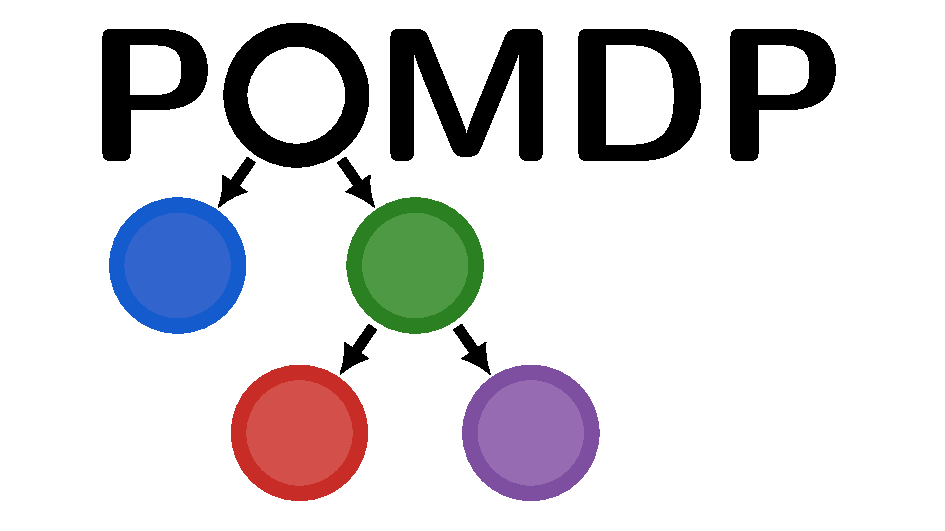
\includegraphics[height=3cm]{images/pomdps_logo.pdf}};
    % \node[xshift=-2cm, yshift=2cm] (img1) at (current page.south east) {\transduration<0-21>{0}\multiinclude[<+->][format=png, graphics={width=\textwidth}]{images/grid-world-animation/gridworld_value_iteration_γ}};
\end{tikzpicture}

\end{frame}

%-------------------------------------------------

\begin{frame}[fragile]{Example problems covered in this course}

Common problems in the literature are used as running examples.

% TODO: Photos.

{\footnotesize
\begin{itemize}
    \item \textbf{$^\text{(MDP)}$ Grid World}: Agent moving around a grid world, looking for rewards.
    \item \textbf{$^\text{(POMDP)}$ Crying Baby}: When to feed a baby, based on crying observations.
    \item \textbf{$^\text{(MDP)}$ 1D Random Walk}: Agent moves around the number line.
    \item \textbf{$^\text{(POMDP)}$ 2D Random Walk}: Estimating state of a moving agent based on observations.
    \item \textbf{$^\text{(MDP)}$ Mountain Car}: Reach a goal up a hill, starting in a valley.
    \item \textbf{$^\text{(MDP)}$ Swinging Pendulum}: Balance a swinging pendulum upright.
\end{itemize}
}

\begin{minipage}[b]{0.18\textwidth}
    \centering
    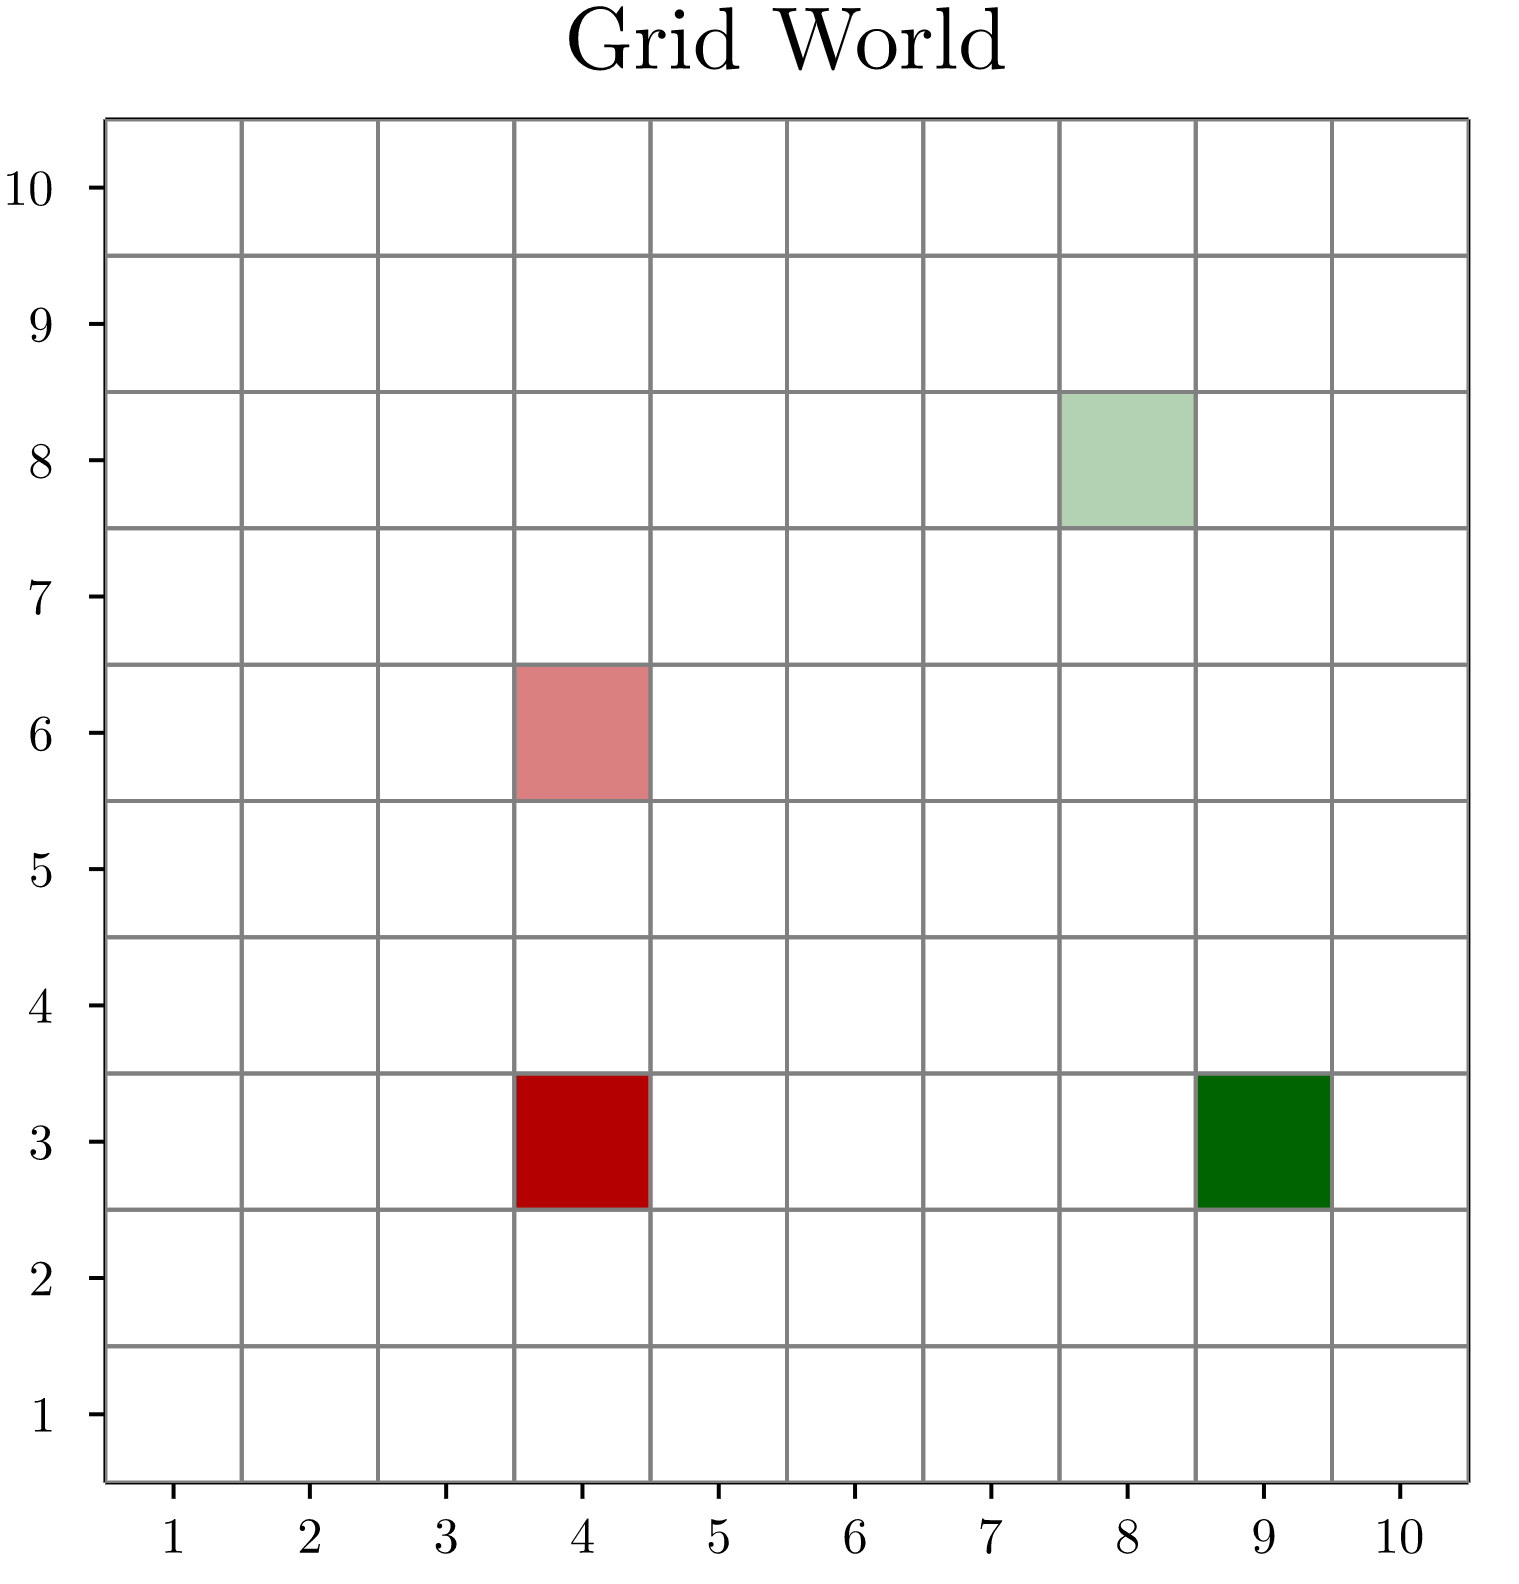
\includegraphics[align=c, width=0.8\textwidth]{images/grid-world.png}
\end{minipage}
\hfill
\begin{minipage}[b]{0.18\textwidth}
    \centering
    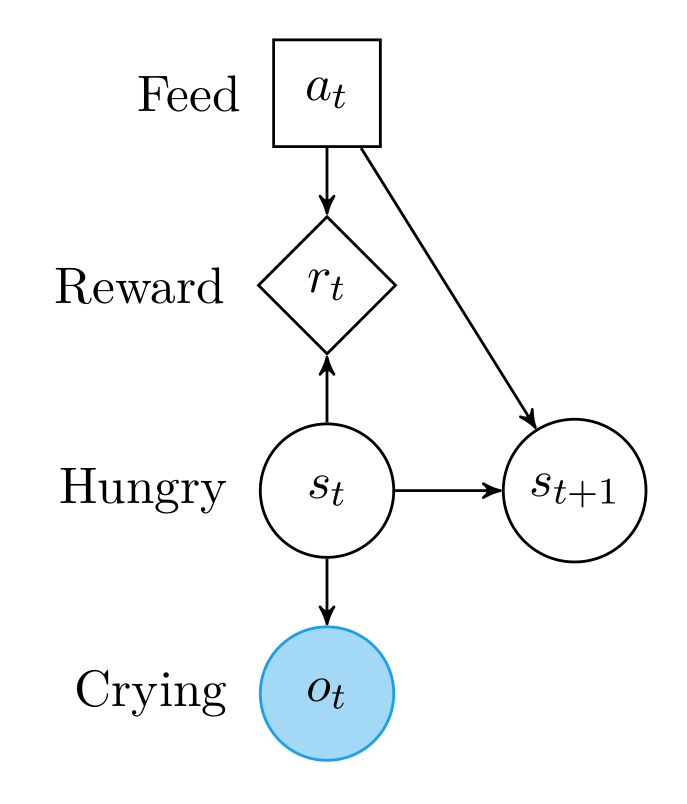
\includegraphics[align=c, width=0.9\textwidth]{images/crying-baby.png}
    % \resizebox{!}{0.3\textheight}{%
    % \begin{tikzpicture}
    %     \node[minimum size=1cm, draw=black, fill=white, circle] (s) {$s_t$};
    %     \node[minimum size=1cm, draw=black, fill=white, circle, right=0.8cm of s] (s2) {$s_{t+1}$};
    %     \node[minimum size=1cm, draw=pastelBlue, fill=pastelBlue!40, circle, below=0.5cm of s] (o) {$o_t$};
    %     \node[minimum size=1cm, draw=black, fill=white, diamond, above=0.5cm of s] (r) {$r_t$};
    %     \node[minimum size=0.8cm, draw=black, fill=white, rectangle, above=0.5cm of r] (a) {$a_t$};
    %     \node[left=0.1 of a, anchor=east] {Feed};
    %     \node[left=0.1 of r, anchor=east] {Reward};
    %     \node[left=0.1 of s, anchor=east] {Hungry};
    %     \node[left=0.1 of o, anchor=east] {Crying};
    %     \draw[->] (s) -- (o);
    %     \draw[->] (s) -- (s2);
    %     \draw[->] (s) -- (r);
    %     \draw[->] (a) -- (r);
    %     \draw[->] (a) -- (s2);
    % \end{tikzpicture}}
\end{minipage}
\hfill
\begin{minipage}[b]{0.18\textwidth}
    \centering
    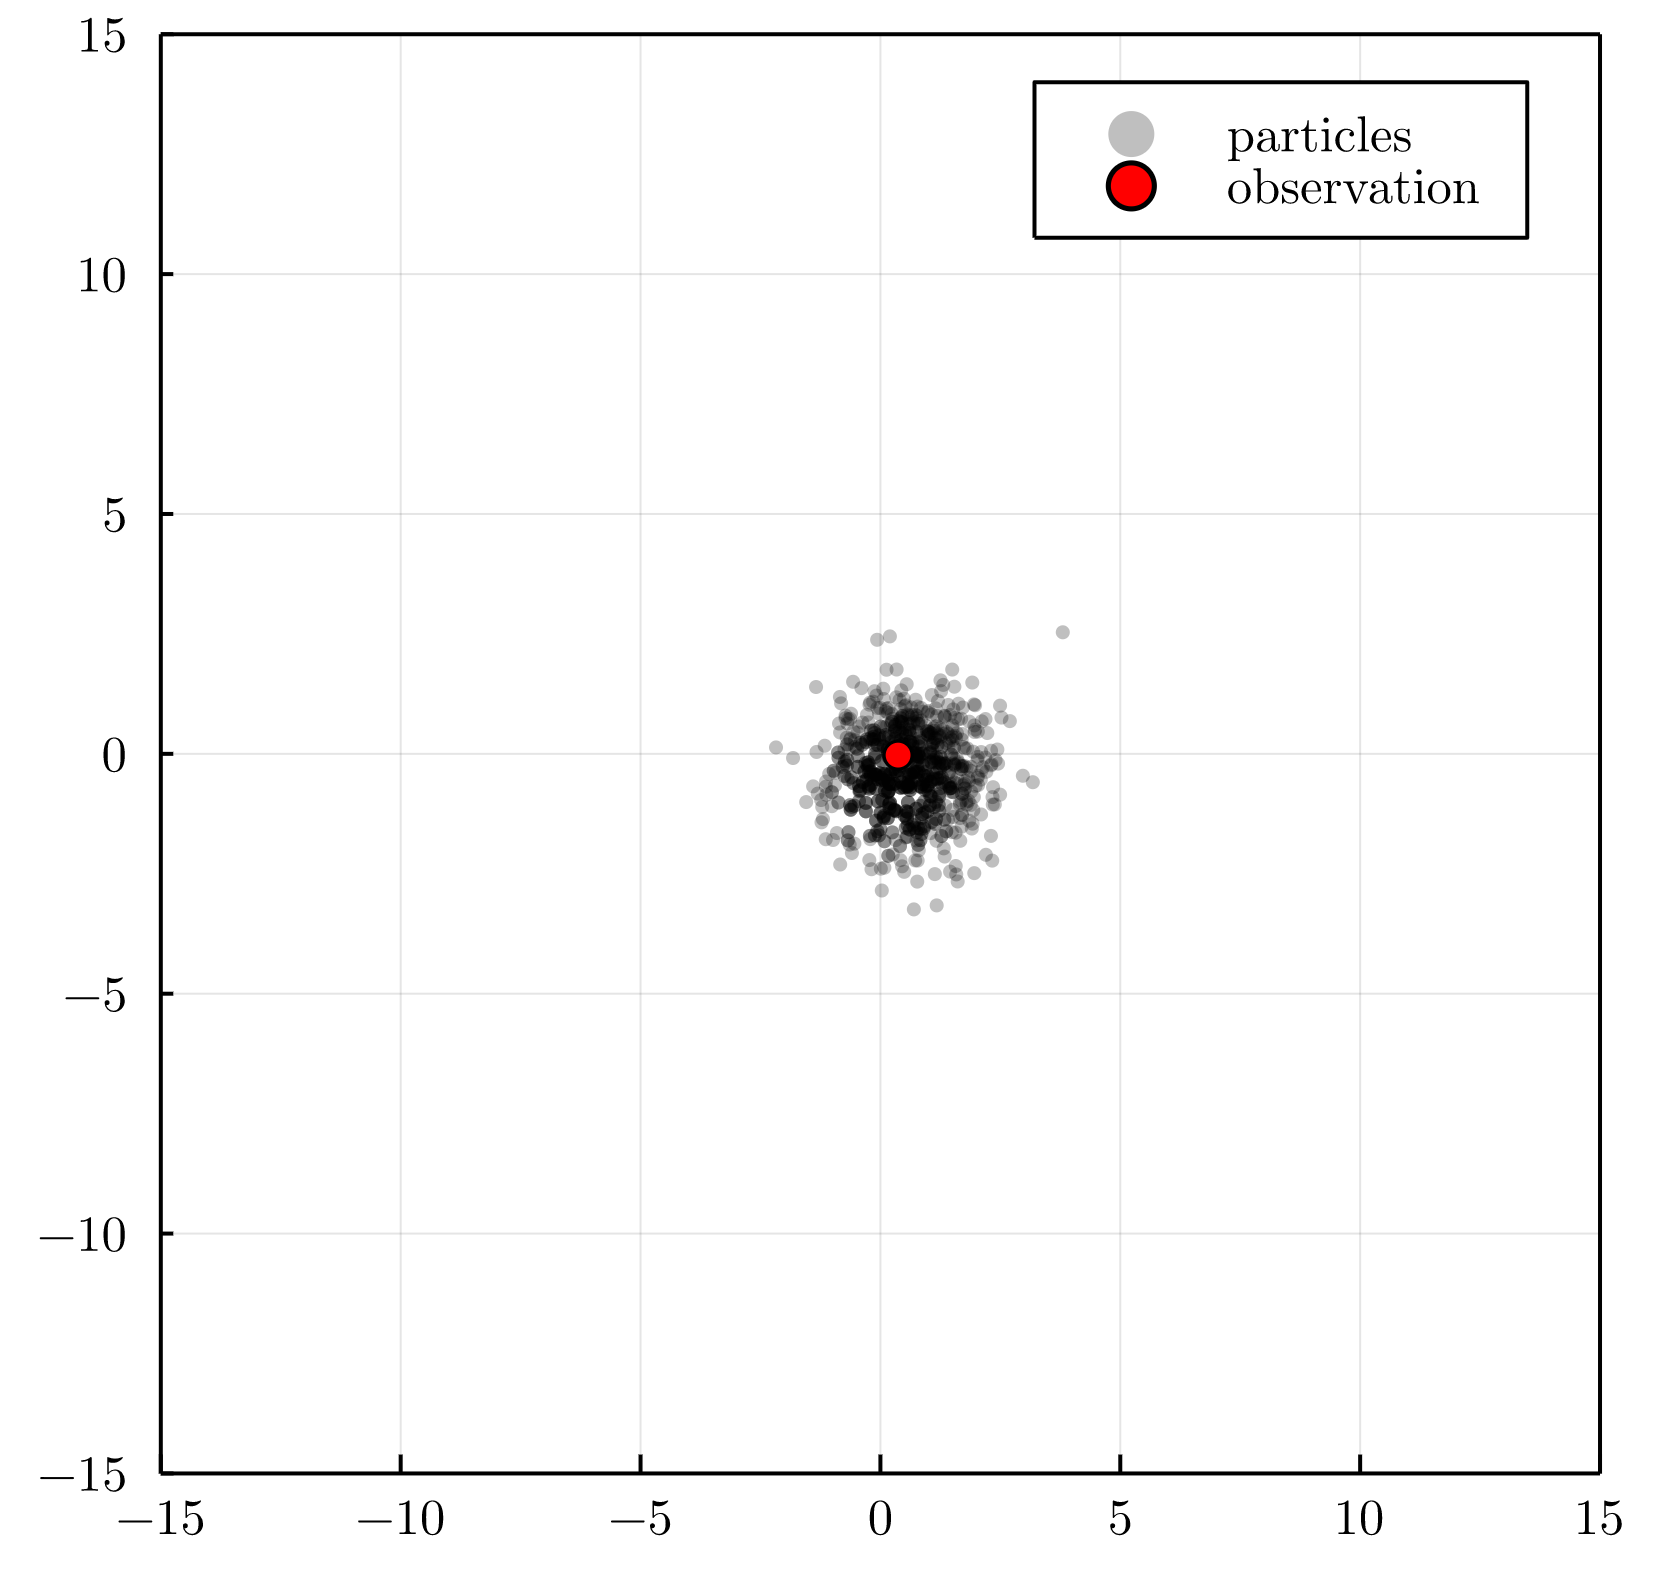
\includegraphics[align=c, width=1.0\textwidth]{images/particle-filter.png}
\end{minipage}
\hfill
\begin{minipage}[b]{0.18\textwidth}
    \centering
    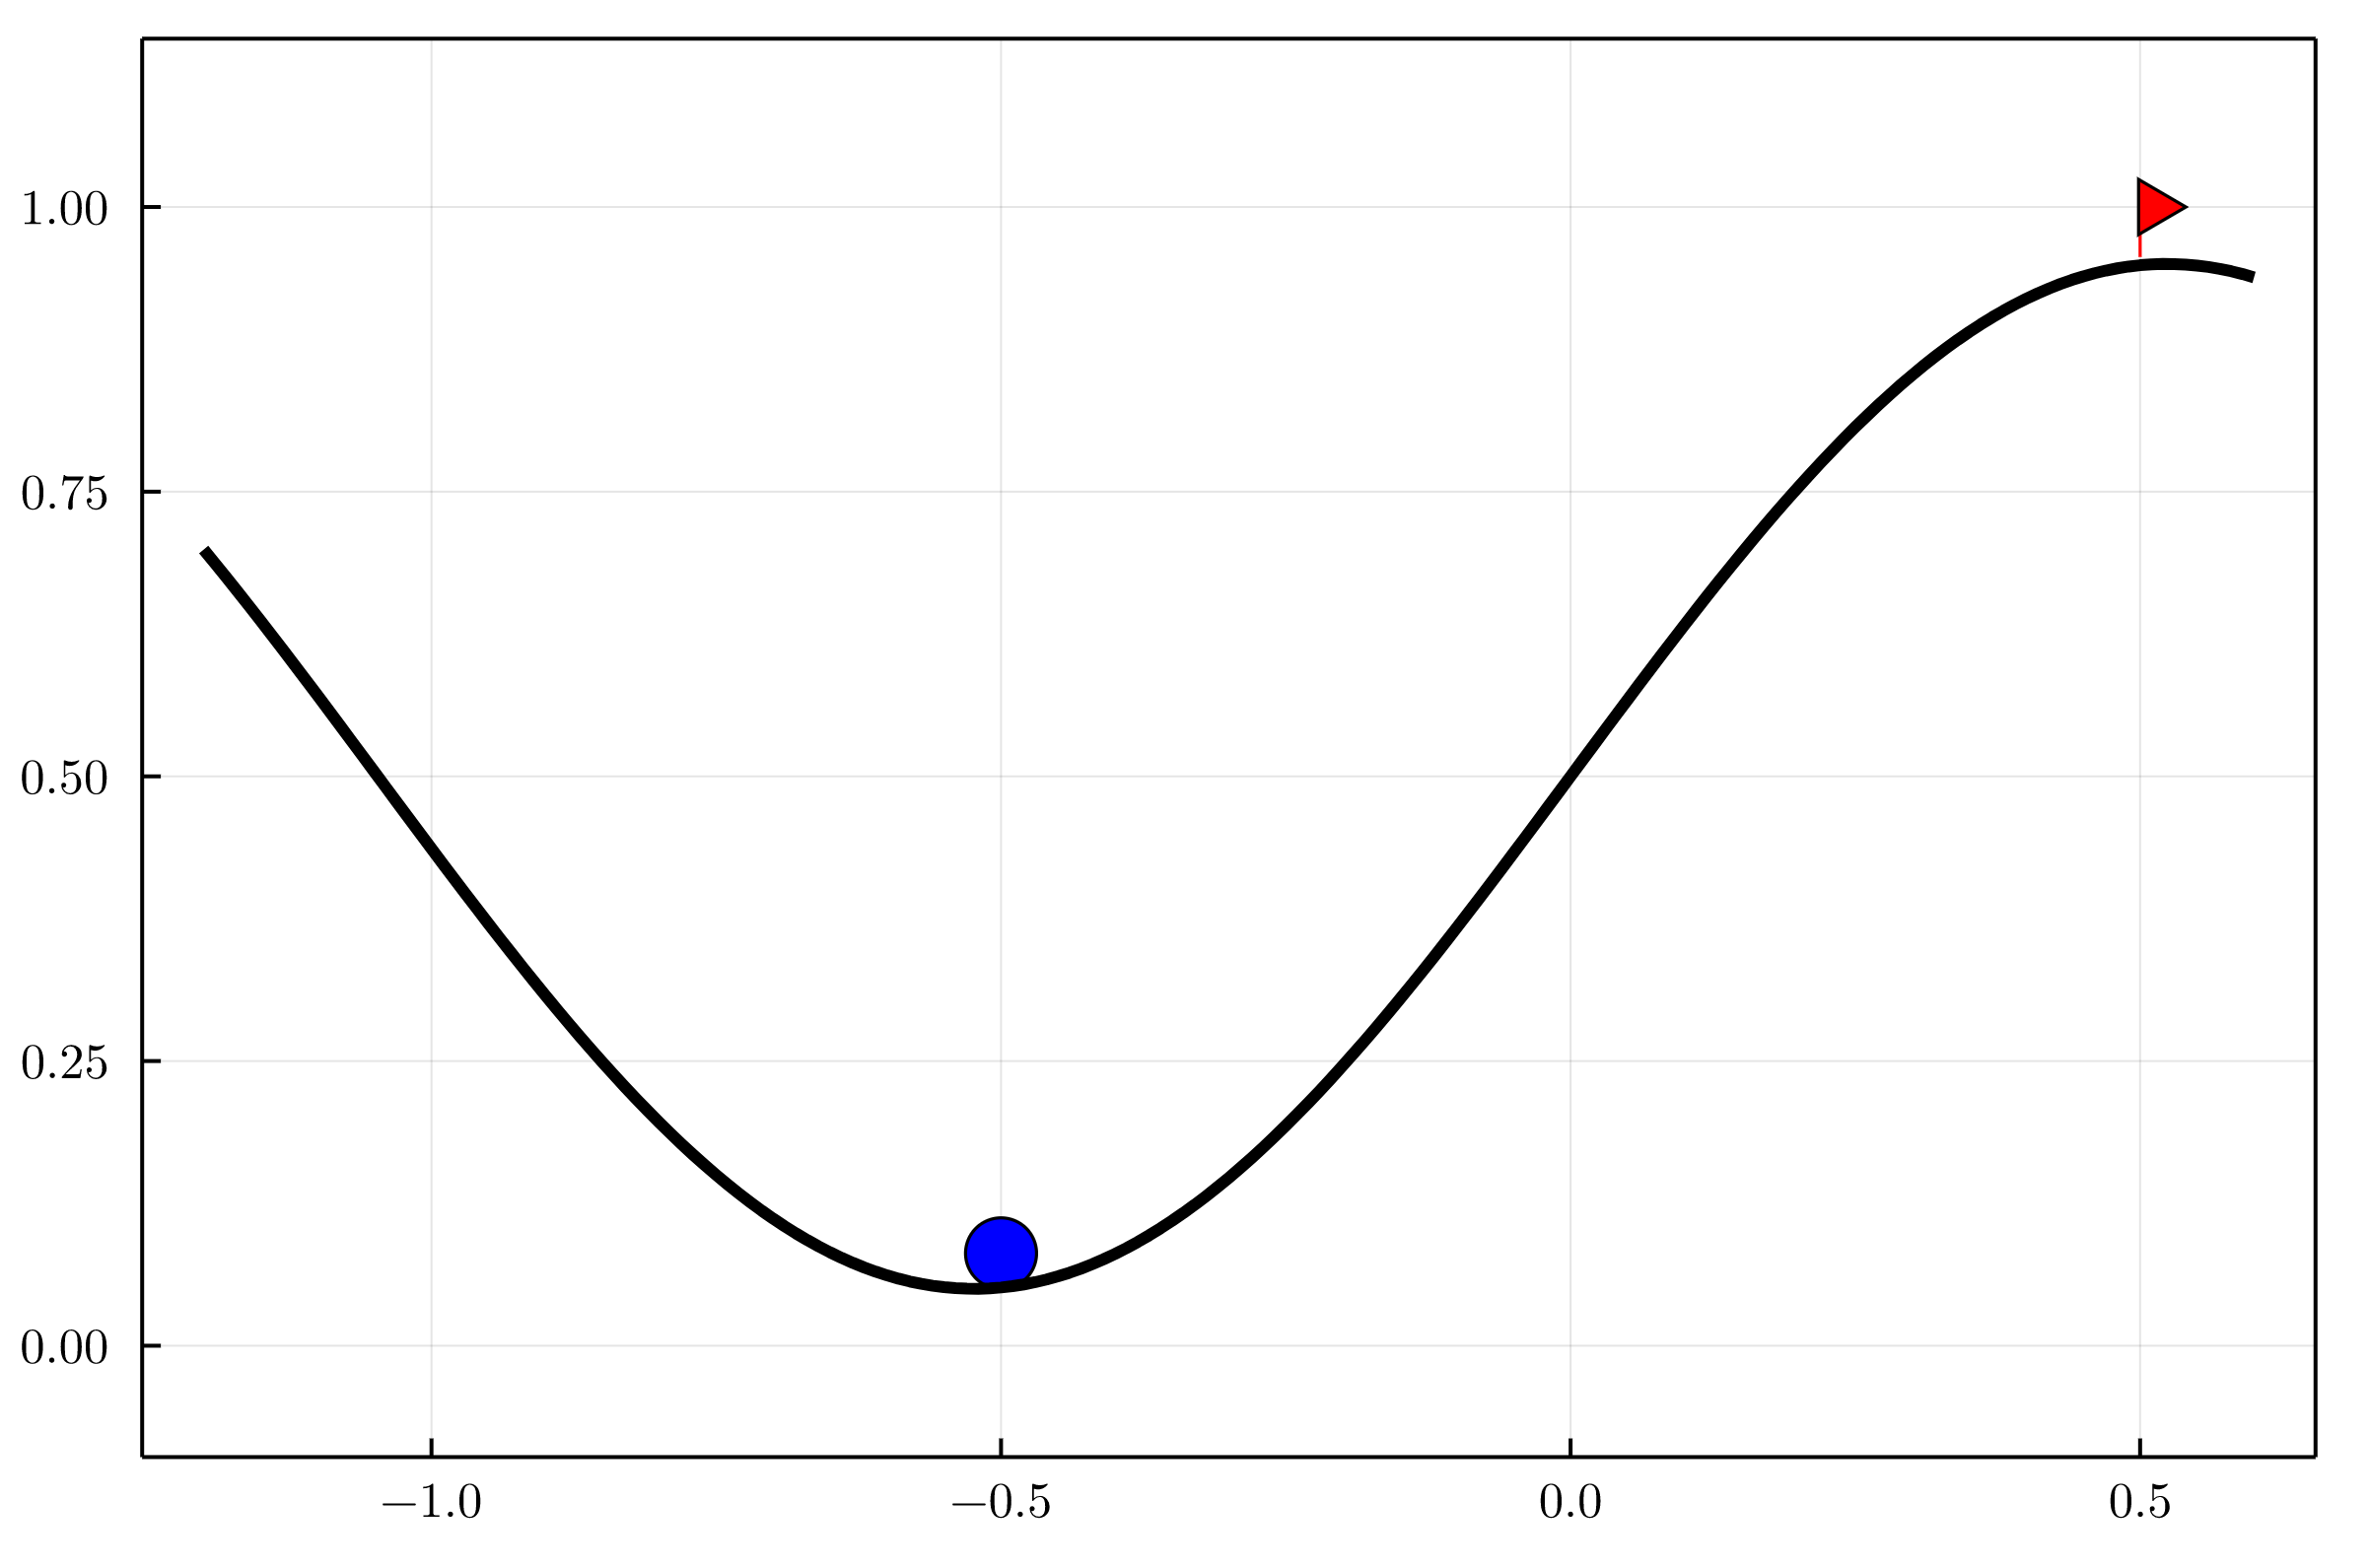
\includegraphics[align=c, width=1.0\textwidth]{images/mountain-car.png}
\end{minipage}
\hfill
\begin{minipage}[b]{0.18\textwidth}
    \centering
    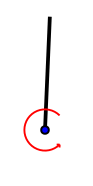
\includegraphics[align=c, width=0.5\textwidth]{images/pendulum.png}
\end{minipage}

\end{frame}

%-------------------------------------------------

\begin{frame}[fragile]{\texttt{POMDPs.jl} package ecosystem}

\begin{highlightblock}
The \texttt{POMDPs.jl} package itself contains the interface to define problem definitions.
\end{highlightblock}

\phantom{}

Other packages provide supporting tools that contain most of the functionality:\footnotemark[1]

\begin{columns}[T,onlytextwidth]
    \begin{column}{0.28\linewidth}
        {\tiny
        \begin{itemize}
            \item {\color{julia_blue}\href{https://github.com/JuliaPOMDP/QuickPOMDPs.jl}{\texttt{QuickPOMDPs.jl}}}
            \item {\color{julia_blue}\href{https://github.com/JuliaPOMDP/POMDPModelTools.jl}{\texttt{POMDPModelTools.jl}}}
            \item {\color{julia_blue}\href{https://github.com/JuliaPOMDP/POMDPPolicies.jl}{\texttt{POMDPPolicies.jl}}}
            \item {\color{julia_blue}\href{https://github.com/JuliaPOMDP/POMDPSimulators.jl}{\texttt{POMDPSimulators.jl}}}
            \item {\color{julia_blue}\href{https://github.com/JuliaPOMDP/POMDPModels.jl}{\texttt{POMDPModels.jl}}}
            \item {\color{julia_blue}\href{https://github.com/JuliaPOMDP/POMDPGallery.jl}{\texttt{POMDPGallery.jl}}}
            \item {\color{julia_green}\href{https://github.com/JuliaPOMDP/BeliefUpdaters.jl}{\texttt{BeliefUpdaters.jl}}}
            \item {\color{julia_green}\href{https://github.com/JuliaPOMDP/ParticleFilters.jl}{\texttt{ParticleFilters.jl}}}
            \item {\color{julia_green}\href{https://github.com/sisl/POMDPModelChecking.jl}{\texttt{POMDPModelChecking.jl}}}
            \item {\color{julia_green}\href{https://github.com/sisl/POMDPStressTesting.jl}{\texttt{POMDPStressTesting.jl}}}
        \end{itemize}
        }
    \end{column}
    \begin{column}{0.36\linewidth}
        {\tiny
        \begin{itemize}
            \item {\color{julia_red}\href{https://github.com/JuliaPOMDP/DiscreteValueIteration.jl}{\texttt{DiscreteValueIteration.jl}}}
            \item {\color{julia_red}\href{https://github.com/JuliaPOMDP/LocalApproximationValueIteration.jl}{\texttt{LocalApproximationValueIteration.jl}}}
            \item {\color{julia_red}\href{https://github.com/JuliaPOMDP/GlobalApproximationValueIteration.jl}{\texttt{GlobalApproximationValueIteration.jl}}}
            \item {\color{julia_red}\href{https://github.com/JuliaPOMDP/MCTS.jl}{\texttt{MCTS.jl}}}
            \item {\color{julia_red}\href{https://github.com/JuliaPOMDP/TabularTDLearning.jl}{\texttt{TabularTDLearning.jl}}}
            \item {\color{julia_red}\href{https://github.com/JuliaPOMDP/DeepQLearning.jl}{\texttt{DeepQLearning.jl}}}
            \item {\color{julia_red}\href{https://github.com/ancorso/Crux.jl}{\texttt{Crux.jl}}}
            \item {\color{julia_purple}\href{https://github.com/JuliaPOMDP/QMDP.jl}{\texttt{QMDP.jl}}}
            \item {\color{julia_purple}\href{https://github.com/JuliaPOMDP/FIB.jl}{\texttt{FIB.jl}}}
        \end{itemize}
        }
    \end{column}
    \begin{column}{0.32\linewidth}
        {\tiny
        \begin{itemize}
            \item {\color{julia_purple}\href{https://github.com/JuliaPOMDP/BeliefGridValueIteration.jl}{\texttt{BeliefGridValueIteration.jl}}}
            \item {\color{julia_purple}\href{https://github.com/JuliaPOMDP/SARSOP.jl}{\texttt{SARSOP.jl}}}
            \item {\color{julia_purple}\href{https://github.com/JuliaPOMDP/BasicPOMCP.jl}{\texttt{BasicPOMCP.jl}}}
            \item {\color{julia_purple}\href{https://github.com/JuliaPOMDP/ARDESPOT.jl}{\texttt{ARDESPOT.jl}}}
            \item {\color{julia_purple}\href{https://github.com/JuliaPOMDP/MCVI.jl}{\texttt{MCVI.jl}}}
            \item {\color{julia_purple}\href{https://github.com/JuliaPOMDP/POMDPSolve.jl}{\texttt{POMDPSolve.jl}}}
            \item {\color{julia_purple}\href{https://github.com/JuliaPOMDP/IncrementalPruning.jl}{\texttt{IncrementalPruning.jl}}}
            \item {\color{julia_purple}\href{https://github.com/JuliaPOMDP/POMCPOW.jl}{\texttt{POMCPOW.jl}}}
            \item {\color{julia_purple}\href{https://github.com/JuliaPOMDP/AEMS.jl}{\texttt{AEMS.jl}}}
            \item {\color{julia_purple}\href{https://github.com/JuliaPOMDP/PointBasedValueIteration.jl}{\texttt{PointBasedValueIteration.jl}}}
        \end{itemize}
        }
    \end{column}
\end{columns}

\footnotetext[1]{\textit{Key}: {\color{julia_blue}Tools}, {\color{julia_green}Extensions}, {\color{julia_red}MDP solvers}, {\color{julia_purple}POMDP solvers}.}

\end{frame}

%-------------------------------------------------

\begin{frame}[fragile]{Other resources}

There are many \textit{excellent} resources on MDPs/POMDPs and reinforcement learning:

{\scriptsize
\begin{itemize}
    \item \textbf{\textit{Algorithms for Decision Making}, Kochenderfer, Wheeler, \& Wray} ({\color{julia_blue}\url{https://algorithmsbook.com/}})
    \item \textbf{\textit{Reinforcement Learning: An Introduction}, Sutton \& Barto} ({\color{julia_blue}\url{http://incompleteideas.net/book/the-book.html}})
    \item \textbf{\textit{POMDPs.jl: A Framework for Sequential Decision Making under Uncertainty}, Egorov, Sunberg, et al., Journal of Machine Learning Research, 2017} ({\color{julia_blue}\url{https://www.jmlr.org/papers/volume18/16-300/16-300.pdf}})
    \item \textbf{Introduction to Reinforcement Learning with David Silver} ({\color{julia_blue}\url{https://deepmind.com/learning-resources/-introduction-reinforcement-learning-david-silver}})
\end{itemize}
}

\end{frame}

%-------------------------------------------------
